\section{Parsing StackOverflow Answers}

\systemname{} allows users to perform queries on answers to over 700,000 Java questions indexed on StackOveflow, an online programming Q\&A site.
On StackOverflow, users pose questions to the community.
Other members provide answers, which are voted to be helpful or unhelpful.
One question can have multiple answers.
For \systemname{}, answers to questions related to a user's query make up the code examples they search through for solutions.

Using StackOverflow as a central corpus for code examples offered three advantages.
First, developers can access the the site's full answer index the StackExchange API, which allows 10,000 queries per day with authentication.
Second, in our own experience we have found StackOverflow to provide high quality answers over a range of topics.
Third, each example is \emph{preformatted} into distinct code and text sections when authored in a StackOverflow markdown editor, making separation of text and code in examples simple.
We restrict ourselves to only Java-related answers on StackOverflow, the programming language with the most questions.

We parse three classes of features from examples:

\emph{Content blocks and types}. 
StackOverflow answers have three types of content (Figure~\ref{fig:so_answer}): explanatory text, source code, and in-code comments.
Explanatory text is wrapped in HTML \emph{\textless{}p\textgreater{}} and \emph{\textless{}li\textgreater{}} elements.
It can be divided into sentences by splitting this content on periods.
Code is wrapped in \emph{\textless{}pre\textgreater{}} elements, which can be divided into lines by the newline character.
In-code comments can be detected through regular expression matching of double-slash and slash-star patterns.

\begin{figure}
 \centering
 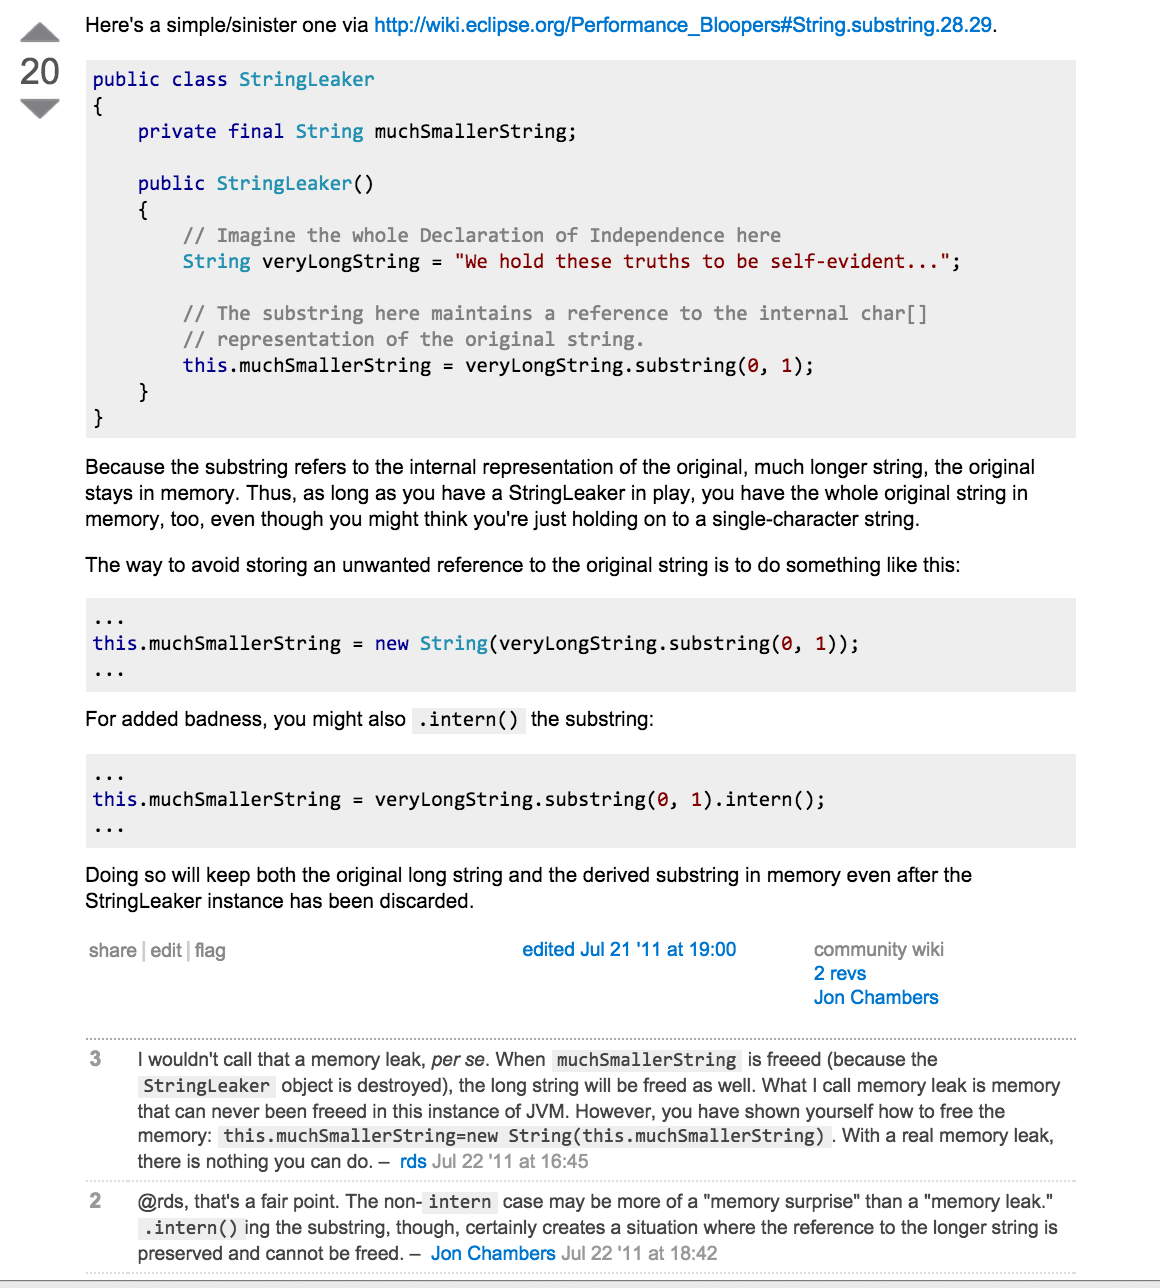
\includegraphics[width=.85\columnwidth]{figures/so_answer}
 \caption{An answer to a Stack Overflow question.  This example contains lines of code, explanatory text, and inline code comments.}
 \label{fig:so_answer}
\end{figure}

\emph{Class usage}.
After extracting content blocks from an answer, we detect classes.
First, we search in the explanatory text for single-word phrases contained within \emph{\textless{}code\textgreater{}} tags.
If the term begins with a capital letter, we assume it to be a Java class.
Second, we perform a regular expression max on the code to detect all class names used in the declaration of a variable, or coupled with a \emph{new} keyword to instantiate an object.

\emph{Concept usage}.
We detect whether examples use concepts learned in the CS1 classroom like loops, functions and objects by using regular expressions for Java keywords, symbols, and sequences of tokens.

We expect that more accurate detection of classes and concepts could be achieved by parsing code examples to their abstract syntax trees and inspecting the nodes of this tree.
However, we note that many code snippets on StackOverflow are incomplete and cannot be compiled.
For this reason, we used regular expression matching to capture class and concept use for this version of \systemname{}.